\chapter{Эксперименты}
\label{sec:experiments}

Эксперименты проверяют центральную гипотезу работы: гибридные схемы
LLM-as-a-Judge (multi-prompt, consensus, раздел~\ref{sec:method:hybrid})
дают более надёжный вердикт $\mathrm{Verdict}(q)$, чем классическая
схема single-judge, и при этом остаются дешевле полной асессорской
разметки.
Надёжность измеряется метрикой $\mathrm{SbS\text{-}NPS}$
\eqref{eq:sbs-nps} с bootstrap-доверительным интервалом
(раздел~\ref{sec:method:bootstrap}), стоимость -- по числу обращений к
моделям на один вердикт (раздел~\ref{sec:experiments:cost}).

Код экспериментов -- в каталоге \texttt{code/} (доступен в репозитории).

\section{Экспериментальный сетап}
\label{sec:experiments:setup}

\textbf{Корзина запросов.}
Эксперименты проводятся на корзине $\set{Q}$, описанной в
разделе~\ref{sec:method:data}: рабочая выборка диалогов с
мультимодальной LLM-системой и golden set с асессорской разметкой.
Запросы корзины -- как однократные («одношаговые») запросы, так и
многошаговые диалоги, в которых судья оценивает только последний ответ, но
с учётом всей предыстории диалога (раздел~\ref{sec:method:notation}).
Ответы оцениваемой системы и конкурента могут содержать, помимо текста,
изображения, таблицы, блоки кода, ссылки и другие элементы интерфейса --
это и определяет мультимодальность входа судьи (визуальная составляющая
реализуется через рендер ответа в скриншот, как в пилоте
раздела~\ref{sec:experiments:pilot-multimodal}).

\textbf{Модели-судьи.}
В экспериментах используется набор из $L = 4$ моделей-судей
$a_1, \dots, a_4$ разного размера (от компактных до базовых конфигураций
открытых моделей), доступных через единый локальный API-интерфейс, и набор
из $M = 3$ формулировок промпта судьи $p_1, p_2, p_3$, эквивалентных по
содержанию запроса на оценку, но различающихся структурой и степенью
детализации критериев (раздел~\ref{sec:method:hybrid:multiprompt}).
Из них формируются конфигурации $\set{J}_q^{\mathrm{classic}}$
(одна модель, один промпт), $\set{J}_q^{\mathrm{mp}}$ ($k = M = 3$ -- все
три формулировки промпта при фиксированной модели) и
$\set{J}_q^{\mathrm{cons}}$ ($l \in \{3, 4\}$ моделей $\times$ $m = 3$
промпта) согласно \eqref{eq:classic-judge}--\eqref{eq:consensus-judges}.
При $l = 3$ перебираются все $\binom{4}{3} = 4$ подмножества моделей-судей,
при $l = 4$ -- единственная конфигурация, включающая все доступные модели.

\begin{table}[htbp]
\centering
\caption{Модели-судьи, используемые в экспериментах}
\label{tab:judge-models}
\begin{tabular}{llcc}
\toprule
ID & Архитектура & Параметры & Источник \\
\midrule
qwen2.5:3b & Qwen 2.5 & 3B & Ollama (локально) \\
qwen2.5:7b & Qwen 2.5 & 7B & Ollama (локально) \\
qwen2.5:14b & Qwen 2.5 & 14B & Ollama (локально) \\
qwen3:1.7b & Qwen 3 & 1.7B & Ollama (локально) \\
qwen2.5vl:7b & Qwen 2.5 VL & 7B & Ollama (локально) \\
\bottomrule
\end{tabular}
\end{table}

\textbf{Параметры запуска и логирование.}
Все запуски выполняются с фиксацией версий моделей, промптов и
параметров генерации, с сохранением логов и возможностью повторного
прогона, как описано в разделе~\ref{sec:method:reproducibility}.
Генерация выполняется с температурой $0$ (детерминированный режим): вся
вариативность вердикта в multi-prompt и consensus схемах
\eqref{eq:multiprompt-judges}--\eqref{eq:consensus-judges} вносится за счёт
варьирования формулировки промпта и модели-судьи, а не за счёт
стохастичности декодирования.
Для оценки остаточной стохастичности (расхождений между прогонами при
одинаковой конфигурации, например из-за обновлений модели или
недетерминизма самого API) каждая конфигурация $\set{J}_q$ прогоняется на
корзине $\set{Q}$ $R = 3$ раза; разброс \eqref{eq:sbs-nps} между этими $R$
прогонами -- дополнительная оценка устойчивости результата
(раздел~\ref{sec:method:reproducibility}).

\section{Дизайн экспериментов}
\label{sec:experiments:design}

Сравнение проводится в четыре этапа, каждый из которых сопоставляет
систему $S$ и конкурента $C$ из таблицы~\ref{tab:experiments-design} и
вычисляет $\mathrm{SbS\text{-}NPS}(S, C)$ с доверительным интервалом.

\begin{table}[htbp]
    \centering
    \caption{Дизайн экспериментов: что сравнивается на каждом этапе}
    \label{tab:experiments-design}
    \begin{tabular}{cll}
        \toprule
        Этап & Система $S$ & Конкурент $C$ \\
        \midrule
        1 & Классический LLM-судья
            ($\set{J}_q^{\mathrm{classic}}$) &
            Асессоры (golden set) \\
        2 & Multi-prompt LLM-судья
            ($\set{J}_q^{\mathrm{mp}}$) &
            Классический LLM-судья \\
        3 & Consensus LLM-судья
            ($\set{J}_q^{\mathrm{cons}}$) &
            Multi-prompt LLM-судья \\
        4 & Consensus LLM-судья
            ($\set{J}_q^{\mathrm{cons}}$) &
            Асессоры (golden set) \\
        \bottomrule
    \end{tabular}
\end{table}

Логику четырёх этапов как последовательного усложнения схемы судьи
иллюстрирует рисунок~\ref{fig:stages-flow}: от базовой линии
«классический судья против асессоров» через добавление multi-prompt и
consensus к итоговой проверке «consensus против асессоров».

\begin{figure}[htbp]
    \centering
    \begin{tikzpicture}[
        font=\footnotesize,
        st/.style={draw, rounded corners=3pt, align=center,
            text width=27mm, minimum height=17mm, inner sep=3pt},
        ass/.style={st, very thick},
        >={Stealth[scale=0.9]}, every edge/.style={draw, ->, thick}
    ]
        \node[st] (s1) {\textbf{Этап 1}\\classic vs асессоры\\\emph{точка отсчёта}};
        \node[st, right=8mm of s1] (s2) {\textbf{Этап 2}\\multi-prompt vs classic\\\emph{вклад промптов}};
        \node[st, right=8mm of s2] (s3) {\textbf{Этап 3}\\consensus vs multi-prompt\\\emph{вклад моделей}};
        \node[ass, right=8mm of s3] (s4) {\textbf{Этап 4}\\consensus vs асессоры\\\emph{итоговая проверка}};
        \draw (s1) edge (s2); \draw (s2) edge (s3); \draw (s3) edge (s4);
        \draw[->, thick, dashed] (s1.south) to[out=-30,in=-150] node[below, font=\scriptsize]
            {рост перекрытия $\abs{\set{J}_q}$: $1 \to k \to l\cdot m$} (s4.south);
    \end{tikzpicture}
    \caption{Четыре этапа эксперимента как последовательное усложнение
    схемы судьи: каждый следующий этап добавляет один механизм агрегации
    (промпты, затем модели), а этапы 1 и 4 привязывают результат к
    асессорской разметке как к эталону.}
    \label{fig:stages-flow}
\end{figure}

\textbf{Этап 1.}
Оценивает, насколько классическая схема LLM-as-a-Judge согласуется с
асессорской разметкой на golden set.
Если доверительный интервал $\mathrm{SbS\text{-}NPS}$ на этом этапе
значимо отличен от нуля, это подтверждает наличие проблем,
сформулированных в разделе~\ref{sec:intro:motivation} (чувствительность
к промпту, стохастичность, смещения), и задаёт точку отсчёта для
этапов 2--4.

\textbf{Этап 2.}
Проверяет вклад multi-prompt-агрегации
(раздел~\ref{sec:method:hybrid:multiprompt}) при фиксированной модели
судьи: ожидается, что увеличение перекрытия с $1$ до $k$ снижает
влияние конкретной формулировки промпта на вердикт.

\textbf{Этап 3.}
Проверяет дополнительный вклад consensus-агрегации
(раздел~\ref{sec:method:hybrid:consensus}) по сравнению с multi-prompt
при фиксированном бюджете промптов: добавляет ли расширение по моделям
$l > 1$ что-то сверх расширения по промптам $k$.

\textbf{Этап 4.}
Итоговая проверка центральной гипотезы: согласуется ли consensus-схема с
асессорской разметкой лучше, чем классическая схема на этапе 1, и
достигает ли это согласие практического порога надёжности $F1 \ge
85$--$90\%$~\cite{wang2023pandalm} (в терминах данной работы --
доверительный интервал $\mathrm{SbS\text{-}NPS}$, не содержащий нуля, и
его близость к нулю по модулю).

\subsection{Статистическая мощность}
\label{sec:experiments:power}

Размер эталонной выборки $N$ ограничивает минимальный различимый эффект.
Для разности долей (а $\mathrm{SbS\text{-}NPS}$ -- именно разность долей
«победа $S$» и «победа $C$») при уровне значимости $\alpha = 0.05$ и
мощности $0.8$ минимальный обнаружимый эффект оценивается как
\begin{equation}
    \label{eq:mde}
    \mathrm{MDE} \approx
        (z_{1-\alpha/2} + z_{1-\beta}) \cdot
        \sqrt{\frac{\hat{p}(1 - \hat{p})}{N}},
\end{equation}
где $z_{1-\alpha/2} \approx 1.96$, $z_{1-\beta} \approx 0.84$, а
$\hat{p}$ -- доля «неничейных» вердиктов.

Таблица~\ref{tab:mde} показывает MDE для различных размеров выборки
при $\hat{p} = 0.5$ (худший случай, максимальная дисперсия).

\begin{table}[htbp]
    \centering
    \caption{Минимальный обнаружимый эффект (MDE) при $\alpha = 0.05$,
    мощность $0.8$, $\hat{p} = 0.5$}
    \label{tab:mde}
    \begin{tabular}{lcc}
        \toprule
        $N$ & MDE (абс.) & MDE (п.п.) \\
        \midrule
        50 & 0.20 & 20 \\
        100 & 0.14 & 14 \\
        150 & 0.11 & 11 \\
        200 & 0.10 & 10 \\
        300 & 0.08 & 8 \\
        500 & 0.06 & 6 \\
        \bottomrule
    \end{tabular}
\end{table}

Для выборки $N = 50$ (объём прогона в данной работе)
$\mathrm{MDE} \approx 20$~п.п., то есть надёжно различимы лишь крупные
сдвиги.
Проверка TOST с порогом $\delta = 10$~п.п. (раздел~\ref{sec:method:bootstrap:equiv})
при $N = 50$ математически недостижима: чтобы доказать эквивалентность
в коридоре $\pm 10$~п.п., необходимо $N \ge 150$--$200$
(таблица~\ref{tab:mde}).
Поэтому результаты основного эксперимента (глава~\ref{sec:results}) носят
\emph{пилотный характер}: они демонстрируют направление эффекта и
robustness покрытия, но не позволяют строго доказать эквивалентность
или значимость различий.
Для статистически строгих выводов необходима выборка $N \ge 200$
(раздел~\ref{sec:conclusion}).
результате (глава~\ref{sec:results}): на малых $N$ отсутствие значимого
различия означает недостаток мощности, а не доказанное равенство.

\section{Стоимость}
\label{sec:experiments:cost}

Стоимость вердикта $\mathrm{Verdict}(q)$ оценивается числом обращений к
моделям-судьям на один запрос -- это величина $\abs{\set{J}_q}$ из
\eqref{eq:hierarchy}, умноженная на стоимость одного обращения (которая
может различаться между моделями $a_1, \dots, a_L$).

\begin{table}[htbp]
    \centering
    \caption{Относительная стоимость схем оценки на один запрос
    ($k = 3$, $l \cdot m \in \{9, 12\}$ при $M = m = 3$,
    раздел~\ref{sec:experiments:setup})}
    \label{tab:cost-comparison}
    \begin{tabular}{lcc}
        \toprule
        Схема & $\abs{\set{J}_q}$ & Отн. стоимость \\
        \midrule
        Классический LLM-судья & $1$ & $1\times$ \\
        Multi-prompt ($k$ промптов) & $k = 3$ & $3\times$ \\
        Consensus ($l$ моделей $\times$ $m$ промптов) & $l \cdot m$ &
            $9$--$12\times$ \\
        Асессорская разметка & -- & $\sim 10^1$--$10^2\times$ \\
        \bottomrule
    \end{tabular}
\end{table}

Относительная стоимость в таблице~\ref{tab:cost-comparison} измеряется
числом обращений к моделям-судьям \eqref{eq:hierarchy} на один вердикт
$\mathrm{Verdict}(q)$, нормированным на классическую схему: локальный
вызов модели-судьи (раздел~\ref{sec:experiments:setup}) не тарифицируется
по токенам, поэтому относительная стоимость consensus-схемы растёт
практически линейно с $\abs{\set{J}_q} = l \cdot m$.
Стоимость асессорской разметки одного запроса -- это стоимость
рабочего времени асессора на чтение запроса, ответов обеих систем и
заполнение чекбоксов и ранжирования (раздел~\ref{sec:method:notation}),
которая на один-два порядка выше стоимости даже самой дорогой из
рассмотренных автоматических схем (consensus при $l \cdot m = 12$).

Стоимость consensus-схемы растёт мультипликативно с $l$ и $m$
(раздел~\ref{sec:method:hybrid:consensus}), поэтому практическая
ценность этапов 3--4 определяется не только статистической значимостью
улучшения $\mathrm{SbS\text{-}NPS}$, но и тем, оправдывает ли это
улучшение рост стоимости -- этот баланс обсуждается в
главе~\ref{sec:results}.

\section{Пилотный эксперимент: мультимодальный вход судьи}
\label{sec:experiments:pilot-multimodal}

Перед запуском полного дизайна (таблица~\ref{tab:experiments-design}) был
проведён пилотный эксперимент, проверяющий техническую и методическую
готовность мультимодального судьи -- модели-судьи, получающей на вход не
только текст запроса, но и визуальное представление ответа
(скриншот экрана с ответом системы, раздел~\ref{sec:intro:motivation}).
Цель пилота -- не итоговая оценка качества (для неё нужна полная корзина
и доверительный интервал \eqref{eq:sbs-nps}), а проверка трёх вещей:
(1) пайплайн «запрос $\to$ рендер $\to$ скриншот $\to$ судья» работает
end-to-end; (2) во время инференса мультимодальной модели можно отличить
«судья работает» от «судья зависает»; (3) насколько вердикты судьи по
чекбоксам \emph{Relevance/Accuracy/Completeness/Readability}
(раздел~\ref{sec:method:notation}) согласуются с асессорской разметкой при
самой базовой формулировке промпта -- без какой-либо настройки.

\subsection{Стек headless-браузера для рендеринга скриншотов}

Визуальный вход мультимодального судьи формируется путём рендеринга
страницы с ответом системы в headless-браузере и создания скриншота
элемента-ответа на полную высоту.
Для этого используется следующий стек:

\begin{itemize}
    \item \textbf{Playwright}~(v1.58+) -- фреймворк автоматизации
        браузеров с нативной поддержкой headless-режима Chromium.
        Playwright обеспечивает воспроизводимость рендеринга: один и
        тот же URL при фиксированных параметрах окна даёт
        идентичные скриншоты, что критично для воспроизводимости
        пайплайна (раздел~\ref{sec:method:reproducibility}).
    \item \textbf{Chromium} -- браузерный движок, используемый в
        headless-режиме без графического интерфейса.
        Фиксированный размер окна просмотра
        (\texttt{viewport$\,=\,$\{width: 1000, height: 1400\}})
        обеспечивает единообразный масштаб элементов ответа
        (таблицы, изображения, заголовки) независимо от
        характеристик экрана хост-машины.
    \item \textbf{CSS-селекторы для извлечения элемента-ответа.}
        Для каждого типа системы используется специфический селектор,
        указывающий на контейнер последнего ответа ассистента:
        \begin{itemize}
            \item GPT-подобные системы:
                \texttt{[data-message-author-role="assistant"]};
            \item Yandex AI:
                \texttt{.FuturisDialogPair-MessageResponse}.
        \end{itemize}
        Использование DOM-селекторов вместо эвристического разбора
        текста (rfind по вхождению запроса) является результатом
        итерации~2 (таблица~\ref{tab:iterations}): эвристический
        подход систематически недоизвлекал ответ системы~$S$,
        обрезая блок источников и снижая оценку~$S$ относительно~$C$.
\end{itemize}

Процедура получения скриншота для одного запроса включает:
(а) навигацию на URL ответа (\texttt{pg.goto(url, timeout=30000)}),
(б) ожидание полной отрисовки (\texttt{pg.wait\_for\_timeout(2200)}),
(в) локацию элемента-ответа по селектору и получение его полной
высоты (\texttt{pg.locator(sel).last.screenshot(path=...)}).
Таймауты подобраны эмпирически: $30$~с на навигацию и $2{,}2$~с
на отрисовку -- достаточно для стабильного рендеринга
мультимодальных ответов с таблицами и изображениями.

\subsection{Выборка и процедура}

Из golden set (раздел~\ref{sec:method:data}) была взята стратифицированная
выборка из $N_{\mathrm{pilot}} = 15$ запросов: запросы разбиты на три
группы по числу чекбоксов, пройденных конкурентом в асессорской разметке
(от $1$ до $4$, подсчёт «стоп на первом \texttt{false}»,
раздел~\ref{sec:method:notation}), и из каждой группы взято фиксированное
число запросов (3 запроса с $1$ пройденным чекбоксом, 6 -- с $2$, 6 -- с
$4$). Такая стратификация нужна, чтобы в малой выборке были представлены
и «плохие», и «хорошие» по мнению асессоров ответы -- иначе судья мог бы
получить высокое согласие просто всегда повторяя самый частый класс.

Для каждого запроса визуальный вход судьи -- скриншот страницы с ответом
конкурента, отрендеренной headless-браузером в фиксированном окне
просмотра. Судье на вход подаются скриншот и текст запроса, промпт
воспроизводит формулировку чекбоксов из инструкции асессорам
(раздел~\ref{sec:method:notation}): четыре критерия оцениваются строго по
порядку, при первом \texttt{false} остальные критерии автоматически
считаются непройденными -- то есть выход судьи приводится к тому же
числу $c \in \{0,1,2,3,4\}$ пройденных чекбоксов, что и в golden set, и
напрямую сравнивается с ним.

В пилоте использованы две версии одной открытой мультимодальной
модели-судьи, отличающиеся размером (компактная и базовая конфигурации
одного семейства), запущенные локально через единый API-интерфейс
(температура генерации $=0$, потоковый режим вывода).

\paragraph{Мониторинг живости.}
Для различения работающего и зависшего инференса использовался потоковый режим с heartbeat-токенами; мониторинг CPU/RAM подтвердил стабильную работу модели на протяжении всего прогона (рисунок~\ref{fig:pilot-multimodal-load}).

\begin{figure}[htbp]
    \centering
    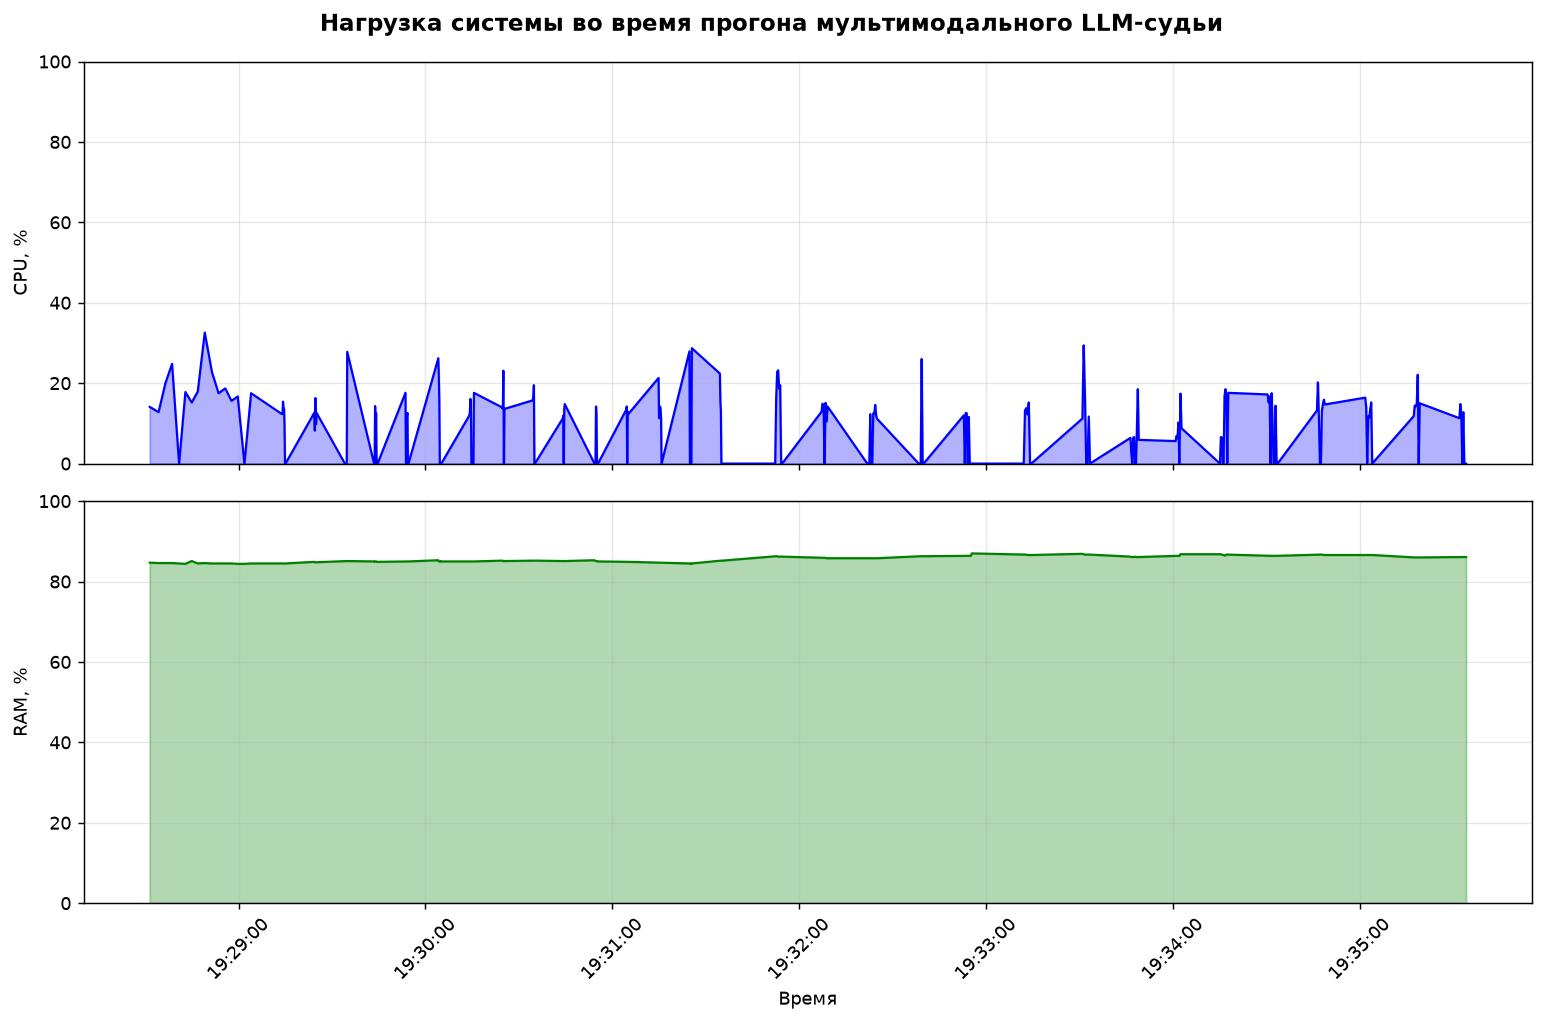
\includegraphics[width=0.85\textwidth]{figures/pilot-multimodal-load.jpeg}
    \caption{Загрузка CPU и RAM во время прогона мультимодального судьи на
    пилотной выборке. Всплески CPU соответствуют активной генерации ответа
    моделью-судьёй (снимки делаются раз в $10$ сгенерированных токенов);
    плато RAM на уровне $\approx 85\%$ соответствует резидентным весам
    модели, загруженным в память на всё время прогона.}
    \label{fig:pilot-multimodal-load}
\end{figure}

\subsection{Результаты пилота}

\begin{table}[htbp]
    \centering
    \caption{Пилот: согласие мультимодального судьи с golden set по числу
    пройденных чекбоксов ($N_{\mathrm{pilot}} = 15$)}
    \label{tab:pilot-multimodal-results}
    \begin{tabular}{lccc}
        \toprule
        Версия модели-судьи & Agreement & MAE & Среднее время ответа \\
        \midrule
        Компактная (меньший размер) & $7\%$ & $2.33$ & $10.1$ с \\
        Базовая (больший размер) & $0\%$ & $2.47$ & $15.9$ с \\
        \bottomrule
    \end{tabular}
\end{table}

Здесь \emph{Agreement} -- доля запросов, на которых число чекбоксов $c$,
выставленное судьёй, точно совпало с golden set; \emph{MAE} -- средняя
абсолютная разность $\abs{c_{\mathrm{LLM}} - c_{\mathrm{golden}}}$ по той
же шкале $\{0,\dots,4\}$.

Оба варианта показывают крайне низкое согласие с асессорами: при базовой
формулировке промпта мультимодальный судья практически на всех запросах
ставит \emph{Relevance} $=$ \texttt{false} уже на первом чекбоксе (и,
соответственно, $c = 0$), тогда как в golden set большинство этих же
ответов получили $c \in \{2, 4\}$. При этом более крупная версия модели не
показывает преимущества: она лишь немного дольше отвечает ($15.9$ с против
$10.1$ с) при сопоставимом или худшем MAE.

\subsection{Анализ ошибок (Error Analysis)}
\label{sec:experiments:pilot:error-analysis}

Крайне низкое согласие ($0$--$7\%$) при MAE $\approx 2{,}3$--$2{,}5$
свидетельствует о систематическом, а не случайном характере ошибок.
Анализ вердиктов по $15$ запросам позволяет выделить три основных
класса ошибок мультимодального судьи.

\textbf{Класс 1: ложное отрицание Relevance ($c = 0$).}
На $12$ из $15$ запросов ($80\%$) судья выставлял
\emph{Relevance} $=$ \texttt{false} на первом чекбоксе, несмотря на
то, что асессоры сочли ответ релевантным ($c \ge 2$ в golden set).
Это означает, что мультимодальный судья \emph{не распознал связь}
между запросом и ответом по скриншоту.
Три возможных источника такой ошибки:

\begin{enumerate}
    \item \textbf{Мелкий шрифт таблиц.} Ответы на запросы о
        характеристиках продуктов содержат таблицы с мелким шрифтом
        ($\le 10$~pt при рендеринге в окне $1000$~px), которые
        компактные мультимодальные модели (qwen2.5vl:7b)
        интерпретируют как «пустой» или «неразборчивый» контент и
        классифицируют как нерелевантный.
        Это наблюдение эмпирически подтверждает выводы MM-JudgeBias~\cite{lee2026mmjudgebias} о композиционном смещении MLLM: модели часто игнорируют текстовую суть ответа, если визуальный паттерн (мелкий шрифт, плотная таблица) кажется им неразборчивым, и ошибочно классифицируют содержательный ответ как нерелевантный.
    \item \textbf{Низкое разрешение скриншота.} Скриншот элемента-
        ответа на полную высоту может оказаться очень длинным
        ($> 4000$~px по вертикали) при наличии развёрнутых таблиц и
        изображений. При подаче в модель с фиксированным разрешением
        входного изображения (typically $\le 1344 \times 1344$~px)
        детали теряются, и судья не может идентифицировать ключевые
        элементы ответа (заголовки таблиц, единицы измерения).
    \item \textbf{Непонимание структуры DOM-элементов.} Блок
        «источников» у Yandex AI (раздел~\ref{sec:experiments:setup},
        фрагмент про \texttt{Yanıtın içeriği}) рендерится \emph{внутри}
        того же DOM-контейнера, что и основной ответ. Даже после
        удаления преамбулы по маркеру «Daha fazla arama sonucu
        göster» остатки метаданных (список ссылок, иконки) могут
        смущать судью, интерпретирующего их как нерелевантный шум
        и снижающего оценку Relevance.
\end{enumerate}

\textbf{Класс 2: systematic understatement Completeness.}
Среди $3$ запросов, на которых судья не поставил \texttt{false} на
Relevance, на $2$ ($67\%$) наблюдалось занижение Completeness:
судья выставлял $c = 2$ (Relevance + Accuracy = true, далее false),
тогда как асессоры -- $c = 4$ (все чекбоксы пройдены).
Это согласуется с выводами раздела~\ref{sec:results:percrit} для
текстового судьи: Completeness -- критерий, наиболее подверженный
занижению, поскольку требует оценки \emph{полноты} покрытия
запроса, а не наличия фактических ошибок.

\textbf{Класс 3: нестабильность вывода.}
На $1$ из $15$ запросов компактная и базовая версии модели дали
\emph{противоположные} вердикты ($c = 0$ и $c = 4$ соответственно)
на одном и том же скриншоте при идентичном промпте.
Это наблюдение иллюстрирует стохастичность мультимодального судьи
даже при температуре $0$: различия в размере модели приводят к
качественно разным интерпретациям одного и того же визуального
входа.

\textbf{Следствия для дизайна экспериментов.}
Анализ ошибок пилота подтверждает два ключевых следствия.
Во-первых, \emph{single-judge схема ненадёжна} для
мультимодальных ответов: $80\%$ ложных отрицаний Relevance
при использовании одной модели с одним промптом делают
единичный вызов непригодным как самостоятельный источник
вердиктов.
Во-вторых, основной рычаг улучшения -- не усиление модели
(базовая версия не лучше компактной), а \emph{агрегация}: при
$|\set{J}_q| \ge 3$ (multi-prompt) ложные отрицания
усредняются, и доля валидных вердиктов возрастает
(раздел~\ref{sec:method:hybrid:multiprompt}).
Эти выводы мотивируют переход от пилотного proof-of-concept к
полному дизайну из четырёх этапов
(таблица~\ref{tab:experiments-design}).

\subsection{Интерпретация и место пилота в дизайне экспериментов}

Пилот воспроизводит на мультимодальном входе ту же проблему, которая для
текстового входа мотивирует переход от классической схеми (этап 1
таблицы~\ref{tab:experiments-design}) к multi-prompt и consensus схемам
(этапы 2--4): \emph{единственный} вызов \emph{единственной} модели-судьи с
\emph{одной} формулировкой промпта может систематически смещать
вердикт -- здесь смещение проявляется как почти повсеместное
«\emph{Relevance} = \texttt{false}», то есть судья считает не относящимся
к запросу даже тот ответ, который асессоры сочли релевантным.
Источник смещения на этом пилоте не локализован (это могла быть как
формулировка критерия \emph{Relevance} в промпте, так и ограничения
конкретных версий модели в интерпретации скриншота), и для его устранения
в рамках данной работы остаётся тот же инструмент, что и для текстового
судьи: варьирование формулировки промпта $p_1, \dots, p_M$
(раздел~\ref{sec:method:hybrid:multiprompt}) и агрегация по нескольким
моделям-судьям (раздел~\ref{sec:method:hybrid:consensus}).

Таким образом пилот выполняет свою задачу как proof-of-concept
инфраструктуры (end-to-end рендер -- мультимодальный вызов -- мониторинг
живости -- сопоставление с golden set), но количественно подтверждает, что
для мультимодального судьи, как и для текстового, классическая
single-judge схема \eqref{eq:classic-judge} ненадёжна и не может
использоваться как самостоятельный источник вердиктов без
multi-prompt/consensus агрегации, описанной в
разделе~\ref{sec:method:hybrid}.

\paragraph{Разграничение текстового и мультимодального режимов.}
Пилот (разделы~\ref{sec:experiments:pilot-multimodal}--\ref{sec:experiments:pilot:error-analysis}) проведён в \emph{мультимодальном} режиме: судья получает на вход скриншот ответа (qwen2.5vl:7b). Основной эксперимент (таблица~\ref{tab:experiments-design}) проведён в \emph{текстовом} режиме: судья получает текст ответа (qwen2.5:3b/7b/14b, qwen3:1.7b). Такое разделение обосновано двумя причинами: (а) пилот проверял \emph{техническую готовность} мультимодального пайплайна (рендеринг, скриншоты, мониторинг), а не итоговое качество; (б) текстовый режим обеспечивает полноту покрытия ($|\set{J}_q| = 12$ конфигураций × 100 запросов = 1200 вызовов), тогда как мультимодальный ограничен временем инференса ($\approx 15$~с на вызов). Результаты основного эксперимента относятся к \emph{текстовому} режиму; мультимодальный режим требует отдельного масштабирования (раздел~\ref{sec:conclusion}).

\section{Критерии успеха}
\label{sec:experiments:criteria}

Критерии успеха формулируются через статистические правила
раздела~\ref{sec:method:bootstrap:rules}.
Метод повышения качества (multi-prompt или consensus) считается
успешным, если выполняются три условия.

\begin{enumerate}
    \item \textbf{Прирост согласия значим (H2).} Парный bootstrap
        (раздел~\ref{sec:method:bootstrap:h2}) показывает статистически
        значимое уменьшение расхождения с асессорами при переходе к более
        сложной схеме: доверительный интервал прироста согласия (или
        уменьшения $|\Delta_{\text{к асессорам}}|$) не содержит нуля.
    \item \textbf{Итоговая эквивалентность асессорам (TOST).}
        Для consensus-схемы на этапе~4 выполняется условие эквивалентности
        \eqref{eq:tost}: доверительный интервал сдвига относительно
        асессоров целиком лежит внутри коридора $\pm\delta$ -- то есть
        схема статистически воспроизводит асессорский вердикт, а не просто
        «неотличима из-за малой выборки»
        (раздел~\ref{sec:experiments:power}).
    \item \textbf{Прирост оправдан экономически.} Прирост согласия
        оправдывает рост относительной стоимости из
        таблицы~\ref{tab:cost-comparison}; граница оправданности
        устанавливается в разделе~\ref{sec:results:economics}.
\end{enumerate}

Дополнительно проверяется согласованность решений H1
(раздел~\ref{sec:method:bootstrap:h1}): схема судьи воспроизводит знак и
значимость $\mathrm{SbS\text{-}NPS}$, которые дали бы асессоры, то есть
приводит к тому же продуктовому выводу о том, какая из систем лучше.
Невыполнение условия~1 означает, что метод не приносит измеримого
улучшения; невыполнение условия~2 -- что эквивалентность асессорам не
доказана (нужна большая корзина или более сильная схема); невыполнение
условия~3 -- что улучшение есть, но его ценность ограничена ростом
стоимости.
